% You should title the file with a .tex extension (hw1.tex, for example)
\documentclass[a4paper, 11pt]{article}
\usepackage{fancyvrb}
\usepackage{verbatim}
\usepackage{amsmath}
\usepackage{amssymb}
\usepackage{fancyhdr}
\usepackage{graphicx}

\usepackage[margin=1in]{geometry}
\usepackage{tikz}
\usetikzlibrary{automata,positioning,arrows}

\usepackage[margin=1in]{geometry}
\usepackage{listings}
\usepackage{color}

\definecolor{dkgreen}{rgb}{0,0.6,0}
\definecolor{gray}{rgb}{0.5,0.5,0.5}
\definecolor{mauve}{rgb}{0.58,0,0.82}

\lstset{frame=tb,
	language=Java,
	aboveskip=3mm,
	belowskip=3mm,
	showstringspaces=false,
	columns=flexible,
	basicstyle={\small\ttfamily},
	numbers=none,
	numberstyle=\tiny\color{gray},
	keywordstyle=\color{blue},
	commentstyle=\color{dkgreen},
	stringstyle=\color{mauve},
	breaklines=true,
	breakatwhitespace=true,
	tabsize=3
}

\newcommand{\question}[2] {\vspace{.25in} \hrule\vspace{0.5em}
	\noindent{\bf #1: #2} \vspace{0.5em}
	\hrule \vspace{.10in}}
\renewcommand{\part}[1] {\vspace{.10in} {\bf (#1)}}

\newcommand{\myname}{Possawat Sanorkam}
\newcommand{\myemail}{possawat2017@hotmail.com}
\newcommand{\myhwnum}{3}

\setlength{\parindent}{0pt}
\setlength{\parskip}{5pt plus 1pt}

\pagestyle{fancyplain}
\lhead{\fancyplain{}{\textbf{HW\myhwnum}}}      % Note the different brackets!
\rhead{\fancyplain{}{\myname\\ \myemail}}
\chead{\fancyplain{}{ICCS310}}

\begin{document}
	
	\medskip                        % Skip a "medium" amount of space
	% (latex determines what medium is)
	% Also try: \bigskip, \littleskip
	
	\thispagestyle{plain}
	\begin{center}                  % Center the following lines
		{\Large ICCS310: Assignment \myhwnum} \\
		\myname \\
		\myemail \\
		\today \\
	\end{center}
	
	\question{1}{NFA vs. DFA Expressiveness} %don't delete yet:(}
	
	\part{1} For every $k \geq 1$, there is an NFA with $k+1$ states that recognizes $C_k$.
	
	{\em Proof}: %reverse it -> 
	We want to directly show that there is an NFA with $k+1$ states that recognizes $C_k$. 
	
	Suppose there is $G_k = (Q,\Sigma,\delta,q_0,F)$ and each $G_k$ contains $Q = \{s_0, s_1,...,s_k\}$ with each state showing how many of the last $k$ bits that $G_k$ has seen for every $k \geq 1$. Then, let $\delta(s_0,b) = s_0$, $\delta(s_0,a) = \{s_0,s_1\}$, $\delta(s_{i-1},a) = s_i$ and $\delta(s_{i-1},b) = s_i$ for $2 \leq i \leq k$. So, let $q_0 = s_0$ and $F = \{S_k\}$. $G_k$ starts at $s_0$, and it may process any character until $a$ is found. Once, $a$ is found, fork the processes into two and we will get one process starts on $s_0$ and $s_1$ at the same time. Just keep changing state from $s_1$ to $s_k$ on any character after $a$ is found and $G_k$ can accepts the string if and only if there are exactly $k-1$ characters following $a$. The process dies immediately when the number of string exceeds $k$ after the $a$ we found at $j$ position where $0 \leq j \leq n$ where $n$ is the length of string. Hence, $G_k$ exists for all $k \geq 1$.
	
	Therefore, for every $k \geq 1$, there is an NFA with $k+1$ states that recognizes $C_k$. $\square$
	
	\part{2} If $M$ is a DFA that correctly recognizes $C_k$, then $M$ has at least $2^k$ states.
	
	{\em Proof}: 
	Consider $\Sigma = \{a,b\}$, we have that there are 2 possible characters, which is $a$ or $b$. Then, let $x,y \in \Sigma^*$ where $|x| = |y| = k$ and $x_i \neq y_i$ for some $0 \leq i \leq k$. If $x_i = a$, then $y_i = b$, vice versa. So, we let $z = b^{k-1}$. Then, $z$ distinguishes $x$ and $y$ as exactly one of $xz$ and $yz$ has the $k^{th}$ character from the end as $a$.
	
	Since there are $2^k$ characters of length k, which are all mutually distinguishable by the above argument, any DFA for the language must have at least $2^k$ states.\\\\\\\\\\\\\\\\\\\\\\\\\\\\\\\\\\\\\\\\
	
	\question{2}{Regular or Not} %don't delete yet:(}
	
	\part{1} $L_1 = \{xyx^R | x,y \in \Sigma^*, x \neq \varepsilon\}$ %regular
	
	{\em Proof}: 
	
	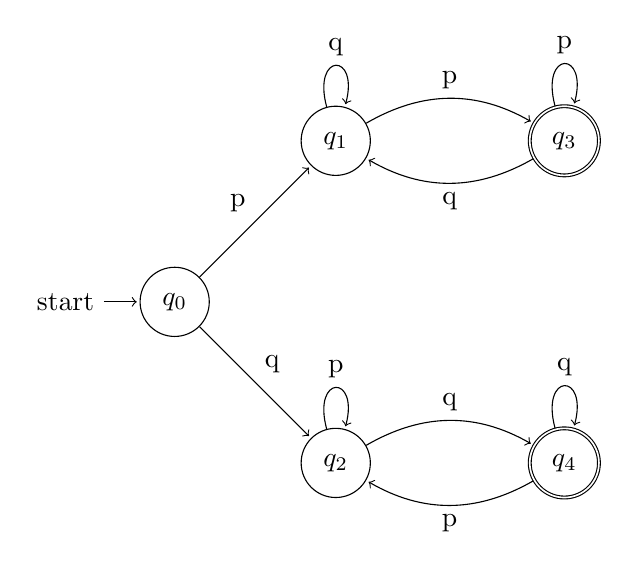
\begin{tikzpicture}[shorten >=1pt,node distance=2cm,auto] 
	\node[state,initial] (q_0)   {$q_0$}; 
	\node[state] (q_1) [above right=of q_0] {$q_1$}; 
	\node[state] (q_2) [below right=of q_0] {$q_2$}; 
	\node[state,accepting] (q_3) [ right=of q_1] {$q_3$}; 
	\node[state,accepting] (q_4) [ right=of q_2] {$q_4$}; 
	\path[->] 
	(q_0) edge  node {p} (q_1)
		  edge  node {q} (q_2)
	(q_1) edge [bend left] node {p} (q_3)
		  edge [loop above] node {q} ()
	(q_2) edge [bend left] node {q} (q_4)
	edge [loop above] node {p} ()
	(q_3) edge [bend left] node {q} (q_1)
		  edge [loop above] node {p} ()
	(q_4) edge [bend left] node {p} (q_2)
	edge [loop above] node {q} ();
	
	\end{tikzpicture}
	
	$S_0$ represents the state where first character is not known.\\
	$S_1$ represents the state where first character is p.\\
	$S_2$ represents the state where first character is q.\\
	$S_3$ represents the state where last character is p, accepted.\\
	$S_4$ represents the state where last character is q, accepted.
	
	The idea is that we do not care what is the given $y$, we only care what character starts first and that character must be the ending character since the reverse of $px$ is $xp$ and $qx$ is $xq$ where $x \in \Sigma^*$.
	
	\part{2} $L_2 = \{xx^R | x \in \Sigma^*, x \neq \varepsilon\}$ %not regular
	
	{\em Proof}: %pumping -> 0 split will break it
	
	
	
	
	
	
	\question{3}{Nonregular}
	
	\part{1} $L = \{10^{n^2} | n \geq 0\}$ %1 follow with 0 n^2 chars 1 4 9
	
	{\em Proof}: %pumping -> 0 split will break it
	Assume for the sake of contradiction that L is regular. Then according to pumping lemma there exist an integer $n$ such that for every string $w$ where $|w| \geq n$, we can break $w$ into three strings $w = xyz$ such that:
	
	-   (1) $xy^iz \in L$ for every $i \geq 0$;
		
	-	(2) $|y| > 0$; and
		
	-	(3) $|xy| \leq n$.
	
	Consider $w = 10^s$ where $s = n^2$. Then, $x = 10000$, $y = 0^j$, and $z = 0^k$. 












	\part{2} $E = \{0^{i}x | i \geq 0\, x \in \{0,1\}^*, \text{and } |x| \leq i\}$ %i 0s follow any char of size 0

	{\em Proof}: %pumping -> 0 split will break it
	
	\question{4}{HackerRank Challenge} 
	
	My username is Possawat2017. All problems solved.
	
	
\end{document}